\documentclass[12pt]{article}


\author{}
\title{}

\usepackage{amsmath}
\usepackage{amsfonts}   % if you want the fonts
\usepackage{amssymb}    % if you want extra symbols
%\usepackage{savetrees}
\usepackage{algorithmic}
\usepackage{graphicx}

\begin{document}
\maketitle

\section{Problem}
\subsection{CFG Basics}
\begin{tabular}{| l l| l}
%  LABEL& EXPR & BASIC BLOCK \\
  \cline{0-1}
  & $x = 100$ & BB0 \\
  & $y = 0$ &  \\
  & goto L2 &  \\
  \cline{0-1}
  L1: & $y = x * y$ & BB1 \\
  & $ \operatorname{if}(x < 50 )$ goto L2 &  \\
  \cline{0-1}
  & $y = x - y$ &  BB2\\
  & goto L3 & \\
  \cline{0-1}
  L2: & $y = x + y$ & BB3 \\
  \cline{0-1}
  L3: & $\operatorname{print}(y)$ & BB4 \\
  & $ \operatorname{if}(y < 1000 )$ goto L1 &  \\
  \cline{0-1}
  & $ \operatorname{if}(x \le 0 )$ goto L5 & BB5  \\
  \cline{0-1}
  L4: & $x = x-1$ & BB6 \\
  & goto L1 & \\
  \cline{0-1}
  L5: & return y & BB7 \\
  \cline{0-1}

\end{tabular}

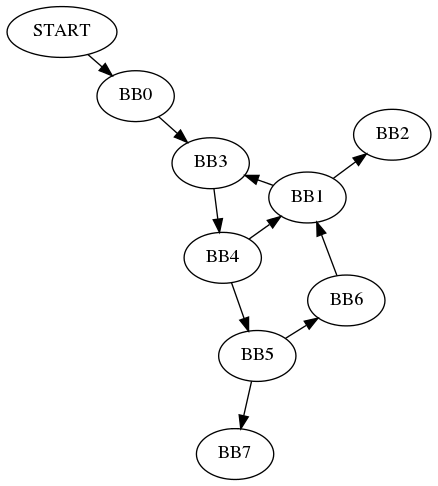
\includegraphics{prob_51_cfg.png}

\subsection{Available Expressions}

\begin{enumerate}
\item
\begin{tabular}{| l| l| l|}
  \hline
  BB & EVAL & KILL \\
  \hline
  1 & $ { d_1, d_2, d_3, d_4}$ & ${ d_5, d_6, d_7, d_8, d_9, d_{10}, d_{11},
      d_{12}} $ \\
  2 & ${ d_5, d_6, d_7 }$ & ${d_9}$ \\
  3 & ${d_8, d_9}$ & ${d_6, d_{12}}$  \\
  4 & ${d_{10}, d_{11}}$  & ${d_8}$  \\
  5 & ${d_{12}}$  & ${d_4}$  \\
  \hline
\end{tabular}

\item
\begin{tabular}{| l| l| l|}
  \hline
  BB & IN & OUT \\
  \hline
  1 & $\emptyset$ & ${ d_1, d_2, d_3, d_4}$ \\
  2 & ${ d_1, d_2, d_3, d_4, d_5, d_6, d_7, d_8, d_9, d_{10}, d_{11}, d_{12}}$
  & ${ d_1, d_2, d_3, d_4, d_5, d_6, d_7, d_8, d_{10}, d_{11}, d_{12}}$ \\
  3 & ${ d_1, d_2, d_3, d_4, d_5, d_6, d_7, d_8,d_{10}, d_{11}, d_{12}}$ & ${
    d_1, d_2, d_3, d_4, d_5, d_7, d_8, d_9, d_{10}, d_{11}}$ \\
  4 & ${ d_1, d_2, d_3, d_4, d_5, d_6, d_7, d_8, d_{10}, d_{11}, d_{12}}$ & ${ d_1, d_2, d_3, d_4, d_5, d_6, d_7, d_9, d_{10}, d_{11}, d_{12}}$ \\
  5 & ${ d_1, d_2, d_3, d_4, d_5, d_6, d_7, d_8, d_9, d_{10}, d_{11}}$ & ${ d_1, d_2, d_3,  d_5, d_6, d_7, d_8, d_9, d_{10}, d_{11}, d_{12}}$ \\
  \hline
\end{tabular}
\end{enumerate}

\subsection{use-without-def}
\begin{enumerate}

\item The elements we are operating on in our analysis is the set of
  definitions, both real definitions and dummy definitions.

\item In this analysis we move from top to bottom, just like in the analysis
  for reaching definitions.

\item Our transfer functions are identical to those in the reaching definition
  analysis. Namely:

  \begin{equation}
    f_b(x) = \operatorname{GEN}_b \cup (\operatorname{IN}[b] - \operatorname{KILL}_b)
  \end{equation}

Where, $\operatorname{GEN}_b$: is the set of definitions exposed in the basic
block $b$. $\operatorname{IN}[b] = \bigcup_{P\in pred\, block}OUT[P]$ and $\operatorname{KILL}_b$ is the
definitions in basic block $b$ that are killed.

\item Our meet operation is set union, $\cup$.

\item We initialize the Exit and Entry nodes as follows:

  \begin{equation}
    \operatorname{OUT}[\operatorname{ENTRY}] = {d^{dummy}_i| i \in
      \operatorname{vars}}
  \end{equation}

  \begin{equation}
    d^{dummy}_i: i := \operatorname{dummy-value}
  \end{equation}

Where $\operatorname{vars}$ is the set of all variables in our program.

\item All of the $IN$ and $OUT$ sets are initialized to $\emptyset$.

\item The ordering does not affect correctness, but because we are chasing
  these dummy definitions down the control flow graph it would be useful to
  use a depth-first traversal.

\item Our analysis will converge because we are dealing with a monotone meet
  function and a finitely sized set.

\item

\begin{algorithmic}
$\operatorname{OUT}[\operatorname{ENTRY}] = {d^{dummy}_i| i \in
      \operatorname{vars}}$
\FORALL {Basic Blocks B other than ENTRY }
    \STATE $\operatorname{OUT}[B]=\emptyset$
\ENDFOR

\WHILE {Changes occur to any other OUT}
    \FORALL  {Basic Blocks B other than ENTRY }
        \STATE $\operatorname{IN}[B] = \bigcup_{P\in pred\, block}OUT[P]$
        \IF {$\operatorname{IN}[B]$ does not contain a dummy variable}
            \STATE \emph{Break}
        \ENDIF

        \STATE $\operatorname{OUT}[B]= \operatorname{GEN}_B \cup (\operatorname{IN}[B] - \operatorname{KILL}_B)$
        \IF {$\operatorname{GEN}_B$  used a dummy variable}
            \STATE Flag use-without-def
        \ENDIF
    \ENDFOR
\ENDWHILE


\end{algorithmic}


\end{enumerate}



\end{document}
